\documentclass[
  bibliography=totoc,
  captions=tableheading,
  titlepage=firstiscover,
]{scrartcl}\usepackage{scrhack}\usepackage[aux]{rerunfilecheck}
\usepackage{amsmath}
\usepackage{amssymb}
\usepackage{mathtools}
\usepackage{fontspec}
\recalctypearea{}
\usepackage{polyglossia}
\setmainlanguage{english}
\usepackage[
  math-style=ISO,
  bold-style=ISO,
  sans-style=italic,
  nabla=upright,
  partial=upright,
  warnings-off={
    mathtools-colon,
    mathtools-overbracket,
  },
]{unicode-math}
\setmathfont{Latin Modern Math}
\setmathfont{XITS Math}[range={scr, bfscr}]
\setmathfont{XITS Math}[range={cal, bfcal}, StylisticSet=1]
\usepackage[
  locale=DE,
  separate-uncertainty=true,
  per-mode=symbol-or-fraction,
]{siunitx}
\usepackage[
  version=4,
  math-greek=default,
  text-greek=default,
]{mhchem}
\usepackage[autostyle]{csquotes}
\usepackage{xfrac}
\usepackage{rotating}
\usepackage{float}
\floatplacement{figure}{htbp}
\floatplacement{table}{htbp}
\usepackage[
  section,
  below,
]{placeins}
\usepackage{pdflscape}
\usepackage[
  labelfont=bf,
  font=small,
  width=0.9\textwidth,
]{caption}
\usepackage{subcaption}
\usepackage{graphicx}
\usepackage{grffile}
\usepackage{booktabs}
\usepackage{microtype}
\usepackage[
  backend=biber,
]{biblatex}
\addbibresource{lit.bib}
\addbibresource{programme.bib}
\usepackage[
  unicode,
  pdfusetitle,
  pdfcreator={},
  pdfproducer={},
]{hyperref}
\usepackage[europeanresistors]{circuitikz}
\usepackage{tikz-feynman}
\usepackage{bookmark}
\usepackage[shortcuts]{extdash}
\author{
  Kevin Mika\\
  \href{kevin.mika@tu-dortmund.de}{kevin.mika@tu-dortmund.de}%
  \texorpdfstring{\and}{,}
  Noah Krystiniak\\
  \href{noah.krystiniak@tu-dortmund.de}{noah.krystiniak@tu-dortmund.de}%
}
\publishers{TU Dortmund – Faculty of Physics}
\subject{51}
\title{Operational amplifier}
\date{%
  Execution: 13.11.2018
}
\usepackage{fancyhdr}
\usepackage{csvsimple}
\pagestyle{fancy}
\rhead{V51 Operational amplifier}
\lhead{Kevin Mika, Noah Krystiniak}
\begin{document}
\maketitle
\tableofcontents
\thispagestyle{empty}
\newpage
\setcounter{page}{1}
%\section{Theorie}
\subsection{Operational Amplifier in General}
The operational amplifier (=OA) is a DC-coupled difference amplifier and a general circuit is shown in
(@@).
\begin{figure}[H]
  \centering
  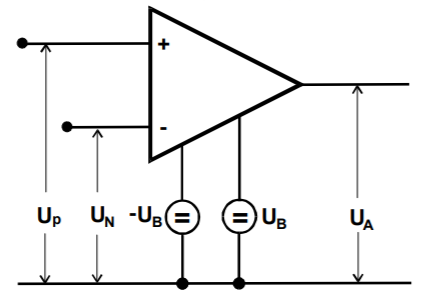
\includegraphics[scale=1]{V51Bilder/t1.png}
  \caption{General principle of an operational amplifier (operating voltages $\pm U_B$ are often left out)} \label{fig:t1} \cite{1}
\end{figure}
\noindent
With the amplification value $V$, the output voltage is
\begin{equation}
U_A = V(U_p - U_N) \label{eq:1}
\end{equation}
as long as it does not exceed the operating voltage $\pm U_B$. If it does, then $U_A = \pm U_B$ applies, depending on whether
the negative or positive value is exceeded. $V$ usually is a very large value, so minimal differences of the input voltages are enough
to exceed the operating range $\pm U_B$. Furthermore $U_A$ is in phase with the "+" - input making this the non-inverting input, and out of phase
with the "-" - input making this the inverting input.
\\
\noindent
For an ideal OA some characteristics are: infinite neutral amplification $V$ and input resistances $r_e$, and an output resistance $r_a$ of zero.
However for the real OA these values do not apply, but instead $V$ is large compared to one and depends on the frequency, $r_e$ take up large and $r_a$ small values.
For an almost-ideal OA these conditions may result only in small discrepancies on measurements compared to idealistic calculations.

\subsection{Linear Amplifier}
To get an useful operating range for the OA a negative-feedback-branch is needed, meaning that some part of $U_A$ is send back to the inverting input.
In figure (\ref{fig:lin}) a linear amplifier is shown.
\begin{figure}
  \centering
  \begin{circuitikz}
    \draw
    (0, 0) node[op amp] (opamp2) {}
    (opamp2.-) to[R,a=$R_1$] (-4, 0.5)
    (opamp2.-) (-1.5,0.49)--(-1.5,1.5)
    to[R,l=$R_N$] (1.19,1.5)
    to[short] (opamp2.out)
    (opamp2.+) --(-1.19,-1.5)
    ;
    \draw
    (0,-1.5)--(-4,-1.5)
    (0,-1.5)--(1.2,-1.5)
    ;
    \draw[<|-|>]
    (-4,-1.5)--(-4,0.49);
    \draw[<|-|>]
    (1.2,-1.5)--(opamp2.out)
    ;
    \draw[<|-|>]
    (-1.5,0.49)--(-1.5,-1.5)
    ;
    \node [right, align=left] at (-4,-0.5){$U_1$};
    \node [left, align=left] at (-1.5,-0.5){$U_N$};
    \node [right, align=left] at (1.2,-0.7){$U_A$};

  \end{circuitikz}
  \caption{Negative feedback inverting linear amplifier}
  \label{fig:lin}
\end{figure}
The negative feedback reduces the total amplification of the circuit but expands the operating range. Calculations for an ideal OA ($V = \infty = r_e$), using Kirchhoff's current law,
lead to
\begin{align}
  \frac{U_1}{R_1} + \frac{U_A}{R_N} &= 0  \label{eq:2.1}\\
  V' &= -\frac{R_N}{R_1} \label{eq:2.2} \ .
\end{align}
However, the non-idealistic characteristics will have a small influence on this equation. If the impact of a finite neutral amplification $V$ on the
amplification value $V'$ is calculated through with equation (\ref{eq:1}) and figure (\ref{lin}) a connection between $V$ and $V'$ is found
\begin{equation}
  \frac{1}{V'} \approx \frac{1}{V} + \frac{R_1}{R_N} \ . \label{eq:3}
\end{equation}
Now it becomes clear that for $V \gg \frac{R_N}{R_1}$ equations (\ref{eq:2.2}) and (\ref{eq:3}) are about the same. Concluding this, the larger the negative feedback the smaller the amplification value
and the more precisely equation (\ref{eq:2.2}) applies. Also this leads to the OA working more stable at lower amplifications.
\\
\noindent
In figure (\ref{fig:tnu}) the frequency responses between  an OA with and without negative feedback are compared to visualise the expanded bandwith by negative feedback.
\begin{figure}[H]
  \centering
  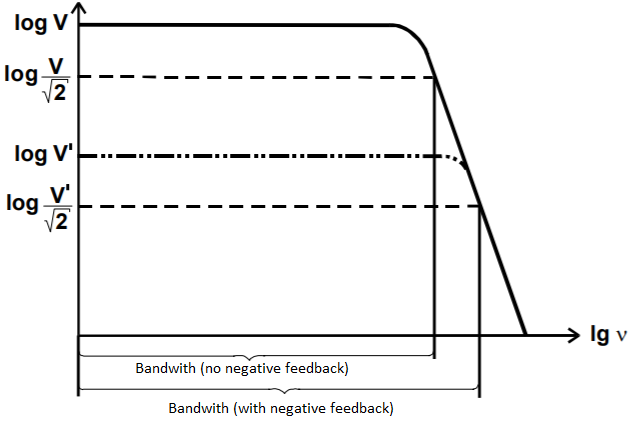
\includegraphics[scale=1]{V51Bilder/t2.png}
  \caption{Frequency response of the linear amplifier} \label{fig:tnu} \cite{1}
\end{figure}
\noindent
Furthermore the product of bandwith and $V'$ is a constant and describes the transit frequency where the amplification drops down to 1. This value is independent of the negative feedback.

\subsection{Electrometer Amplifier}
To measure high-resistance voltage sources a large input resistance $r_e$ is needed. Because that is not the case for the linear amplifier, where $r_e \approx R_1$ ($U_N \approx 0$),
the circuit is modified to the electrometer amplifier. Here the input voltage is directly connected to the non-inverting input of the OA. For the ideal OA is $r_e = \infty$ and for the real
OA $r_e \approx \SI{20}{\giga\ohm}$. \\
\noindent
\begin{figure}
  \centering
  \begin{circuitikz}
    \draw
    (0,0) node[op amp](oplol) {}
    ;
    \draw
    (-2,3)--(1.2,3)
    to[R,l=$R_1$] (1.2,1.5) to[R,l=$R_N$] (oplol.out)
    ;
    \draw (1.2,1.5)--(-1.2,1.5)--(oplol.-);
    \draw (1.2,3)--(2.8,3);
    \draw (-2,-0.5)--(oplol.+);
    \draw[<|-|>]
    (-2,-0.5)--(-2,3);
    \draw (1.5,0)--(2.8,0);
    \draw[<|-|>]
    (2.8,0)--(2.8,3);
    \node [left, align=left] at (-2, 1.75){$U_1$};
    \node [right, align=left] at (2.8, 1.5){$U_A$};
  \end{circuitikz}
  \caption{Non-inverting electrometer amplifier.}
  \label{fig:nig}
\end{figure}

\noindent
For an ideal electrometer amplifier the amplification is
\begin{equation*}
V' = \frac{R_N + R_1}{R_1}
\end{equation*}

\subsection{Inverting Integrator}
With the circuit in figure (\ref{fig:integrator}) it is possible to integrate the input voltage $U_1$.
Using Kirchhoff's law on branch point $A$, that
\begin{equation*}
\int I_C dt = C U_A
\end{equation*}
and that
\begin{equation*}
U_1 = U_0 \text{sin}\omega t
\end{equation*}
it follows for the output voltage
\begin{equation*}
U_A = \frac{U_0}{\omega R C} \text{cos}\omega t \ .
\end{equation*}
This means the output voltage is antiproportional to the frequency.
\begin{figure}[H]
  \centering
  \begin{circuitikz}
      \draw
      (0, 0) node[op amp] (opamp) {}
      (opamp.-) to[R,l=$R$] (-3, 0.5)
      (opamp.-) |- (-1, 2) to[C,a=$C$] (1, 2) -| (opamp.out)
      ;
      \draw (1.2,-1.5)--(-1.2,-1.5)--(opamp.+);
      \draw (-1,-1.5)--(-3,-1.50);
      \draw[<|-|>]
      (1.2,-1.5)--(opamp.out)
      ;
      \draw[<|-|>]
      (-3,-1.5)--(-3,0.5)
      ;
      \node [left, align=left] at (-3,-0.50){$U_1$};
      \node [right, align=left] at (1.2,-0.75){$U_A$};
      \node [above left] at (opamp.-){$A$};
  \end{circuitikz}
  \caption{Inverting integrator}
  \label{fig:integrator}
\end{figure}

\subsection{Inverting Differentiator}
With the same considerations as with the inverting integrator, for the inverting differentiator follows
the output voltage
\begin{equation*}
U_A = -\omega RCU_0 \text{cos}\omega t \
\end{equation*}
with $U_A$ being proportional to the frequency.
\begin{figure}[H]
  \centering
  \begin{circuitikz}
      \draw
      (0, 0) node[op amp] (opamp3) {}
      (opamp3.-) to[C,l=$C$] (-3, 0.5)
      (opamp3.-) |- (-1, 2) to[R,a=$R$] (1, 2) -| (opamp3.out)
      ;
      \draw (1.2,-1.5)--(-1.2,-1.5)--(opamp3.+);
      \draw (-1,-1.5)--(-3,-1.50);
      \draw[<|-|>]
      (1.2,-1.5)--(opamp3.out)
      ;
      \draw[<|-|>]
      (-3,-1.5)--(-3,0.5)
      ;
      \node [left, align=left] at (-3,-0.50){$U_1$};
      \node [right, align=left] at (1.2,-0.75){$U_A$};
  \end{circuitikz}
  \caption{Inverted differentiator}
  \label{fig:diff}
\end{figure}
\subsection{Schmitt-Trigger}
In contrast to the previous amplifiers the Schmitt-Trigger uses positive feedback. In figure (\ref{fig:schmitt}) the circuit is shown.
If a certain input voltage is reached the output voltage will jump immediately to $\pm U_B$, depending on whether the input voltage is positive or negative.
This certain voltage is adjusted by the ratio of the resistances and it follows
  \[U_A = \left\{
    \begin{array}{lr}
      + U_B & : U_1 > +\frac{R_1}{R_P}U_B \\
      - U_B & : U_1 < -\frac{R_1}{R_P}U_B
    \end{array}
  \right.
  \]
Notice that as long as $U_1$ does not exceed one of the two trigger voltages $U_A$ will stay at its current value.
The difference $2 U_B \frac{R_1}{R_P}$ between the two trigger values is called switching hysteresis.
\begin{figure}
  \centering
  \begin{circuitikz}
    \draw
    (0, 0) node[op amp] (opamp5) {}
    (opamp5.+) to[R,l=$R_1$] (-4, -0.5)
    (opamp5.+) (-1.5,-0.49)--(-1.5,-1.5)
    to[R,a=$R_p$] (1.19,-1.5)
    to[short] (opamp5.out)
    ;
    \draw
    (opamp5.-)--(-4,0.49)
    ;
    \draw[<|-|>]
    (-4,-0.49)--(-4,0.49);
    \draw[<|-|>]
    (1.2,-1.5)--(opamp2.out)
    ;
    \draw[<|-|>]
    (-1.5,0.49)--(-1.5,-0.49)
    ;
    \node [right, align=left] at (-4,0){$U_1$};
    \node [left, align=left] at (-1.5,0){$U_p$};
    \node [right, align=left] at (1.2,-0.7){$U_A$};

  \end{circuitikz}
  \caption{Schmitt-Trigger}
  \label{fig:schmitt}

\end{figure}

\section{Execution}
In order to determine the frequency response,
a negative feedback operation amplifier as shown in Figure \ref{fig:gegen} is set up,
which is adjusted via the negative feedback branch. The output voltage and the input voltage are graphically displayed on an oscilloscope.
\begin{figure}
  \centering
  \begin{circuitikz}
    \draw
    (0, 0) node[op amp] (opamp2) {}
    (opamp2.-) to[R,a=$R_1$] (-4, 0.5)
    (opamp2.-) (-1.5,0.49)--(-1.5,1.5)
    to[R,l=$R_N$] (1.19,1.5)
    to[short] (opamp2.out)
    (opamp2.+) --(-1.19,-1.5)
    ;
    \draw
    (0,-1.5)--(-4,-1.5)
    (0,-1.5)--(1.2,-1.5)
    ;
    \draw[<->]
    (-4,-1.5)--(-4,0.49);
    \draw[<->]
    (1.2,-1.5)--(opamp2.out)
    ;
    \draw[<->]
    (-1.5,0.49)--(-1.5,-1.5)
    ;
    \node [right, align=left] at (-4,-0.5){$U_1$};
    \node [left, align=left] at (-1.5,-0.5){$U_N$};
    \node [right, align=left] at (1.2,-0.7){$U_A$};

  \end{circuitikz}
  \caption{Feedback inverting linear amplifier.}
  \label{fig:gegen}
\end{figure}
To determine the terminal voltage, use the circuit shown in Figure \ref{fig:gegen} and a non-inverting electrometer amplifier shown in Figure \ref{fig:nig}.
The circuitry is then used to determine the terminal voltage.
\begin{figure}
  \centering
  \begin{circuitikz}
    \draw
    (0,0) node[op amp](oplol) {}
    ;
    \draw
    (-2,3)--(1.2,3)
    to[R,l=$R_1$] (1.2,1.5) to[R,l=$R_N$] (oplol.out)
    ;
    \draw (1.2,1.5)--(-1.2,1.5)--(oplol.-);
  \end{circuitikz}
  \caption{Non-inverting electrometer amplifier.}
  \label{fig:nig}
\end{figure}
Circuit \ref{fig:integrator} is constructed to integrate input signals using the operational amplifier.
\begin{figure}
  \centering
  \begin{circuitikz}
      \draw
      (0, 0) node[op amp] (opamp) {}
      (opamp.-) to[R,l=$R$] (-3, 0.5)
      (opamp.-) |- (-1, 2) to[C,a=$C$] (1, 2) -| (opamp.out)
      ;
  \end{circuitikz}
  \caption{Reverse integrator.}
  \label{fig:integrator}
\end{figure}
In order to differentiate an input signal, the resistor and capacitor in Figure \ref{fig:integrator}
are swapped according to Figure \ref{fig:diff}.
\begin{figure}
  \centering
  \begin{circuitikz}
      \draw
      (0, 0) node[op amp] (opamp3) {}
      (opamp3.-) to[C,l=$C$] (-3, 0.5)
      (opamp3.-) |- (-1, 2) to[R,a=$R$] (1, 2) -| (opamp3.out)
      ;
  \end{circuitikz}
  \caption{Reverse integrator.}
  \label{fig:diff}
\end{figure}
The Schmitt trigger which works as a switch because the output voltage
changes its sign when the input voltage falls under the following condition:
\begin{equation}
  \frac{-R_1}{R_P}U_B
\end{equation}
\begin{figure}
  \centering
  \begin{circuitikz}
    \draw
    (0, 0) node[op amp] (opamp5) {}
    (opamp5.+) to[R,l=$R_1$] (-4, -0.5)
    (opamp5.+) (-1.5,-0.49)--(-1.5,-1.5)
    to[R,a=$R_p$] (1.19,-1.5)
    to[short] (opamp5.out)
    ;
    \draw
    (opamp5.-)--(-4,0.49)
    ;
    \draw[<->]
    (-4,-0.49)--(-4,0.49);
    \draw[<->]
    (1.2,-1.5)--(opamp2.out)
    ;
    \draw[<->]
    (-1.5,0.49)--(-1.5,-0.49)
    ;
    \node [right, align=left] at (-4,0){$U_1$};
    \node [left, align=left] at (-1.5,0){$U_p$};
    \node [right, align=left] at (1.2,-0.7){$U_A$};

  \end{circuitikz}
  \caption{Schmitt-trigger}
  \label{}
\end{figure}

%\section{Evaluation}
All calculations and plots are done by Python 3.6.1.
\subsection{Inverting Linear Amplifier}
Note that the used amplifier inverts the signal, transforming a positive input to a negative output and vice versa, but for this evaluation only the absolute
amplification and voltages are used. \\
\noindent
For the first part the frequency response of the input voltage $U_1$ for a resistance ratio of 10 and 100 were measured.
The grade of amplification is adjusted by choosing a corresponding ratio of $\frac{\text{R}_\text{N}}{\text{R}_\text{1}}$ with
${\text{R}_\text{N}}$ = \SI{100}{\kilo\ohm} and ${\text{R}_\text{1}}$ = \SI{10}{\kilo\ohm} for a theoretical amplification of -10, and
${\text{R}_\text{N}}$ = \SI{20}{\kilo\ohm} and ${\text{R}_\text{1}}$ = \SI{0.2}{\kilo\ohm} for -100. These are theoretical because due
to equation (\ref{eq:3}) the neutral amplification $V$ can have an impact on $V'$ and can be approximated with it. For this $V'$ is taken from the measurement at low frequencies. In tabular (\ref{tab:1}) and tabular (\ref{tab:2})
are the measured data of frequency $\nu$, input voltage $U_1$ and output voltage $U_A$.

\begin{minipage}[t]{0.48\linewidth}
\begin{table}[H]
  \centering
  \caption{Data for $\frac{\text{R}_\text{N}}{\text{R}_\text{1}}$ = 10} \label{tab:1}
  \pgfplotstabletypeset[
  col sep=semicolon,
  every head row/.style={
    before row={\toprule
    },
    after row=\hline
  },
  every last row/.style={after row=\bottomrule},
  columns/0/.style={column name=$\nu$ / kHz, column type=c, fixed zerofill, precision=2},
  columns/1/.style={column name= $U_1$ / mV, column type=c, precision=3},
  columns/2/.style={column name=$U_A$ / V, column type=c, fixed zerofill, precision=2},
  ]{a1.csv}
\end{table}
\end{minipage}
\begin{minipage}[t]{0.48\linewidth}
\begin{table}[H]
  \centering
  \caption{Data for $\frac{\text{R}_\text{N}}{\text{R}_\text{1}}$ = 100} \label{tab:2}
  \pgfplotstabletypeset[
  col sep=semicolon,
  every head row/.style={
    before row={\toprule
    },
    after row=\hline
  },
  every last row/.style={after row=\bottomrule},
  columns/0/.style={column name=$\nu$ / kHz, column type=c, fixed zerofill, precision=2},
  columns/1/.style={column name= $U_1$ / mV, column type=c, precision=1, fixed zerofill},
  columns/2/.style={column name=$U_A$ / V, column type=c, fixed zerofill, precision=2},
  fixed
  ]{a3.csv}
\end{table}
\end{minipage}
\vskip 0.2in
\noindent
Looking at the values for the low frequencies, it can be seen that $V'_{10} = 10$  and $V'_{100} = \frac{2}{0.023}$.
Therefore $V'_{10} = \frac{\text{R}_\text{N}}{\text{R}_\text{1}} = \frac{\SI{100}{\kilo\ohm}}{\SI{10}{\kilo\ohm}}$ satisfies for low frequencies, but $V'_{100} = \frac{\text{R}_\text{N}}{\text{R}_\text{1}} = \frac{\SI{20}{\kilo\ohm}}{\SI{0.2}{\kilo\ohm}}$ does not.
Now with equation (\ref{eq:3}) $V$ can be estimated using $V'_{100} = \frac{2}{0.023}$ and $\frac{\text{R}_\text{N}}{\text{R}_\text{1}} = 100$ to
\begin{equation*}
  V = 666,67 \ .
\end{equation*}
\\ \noindent
In figure (\ref{fig:1}) and figure (\ref{fig:2}) is a graphical representation of the data.
\begin{figure}
  \centering
  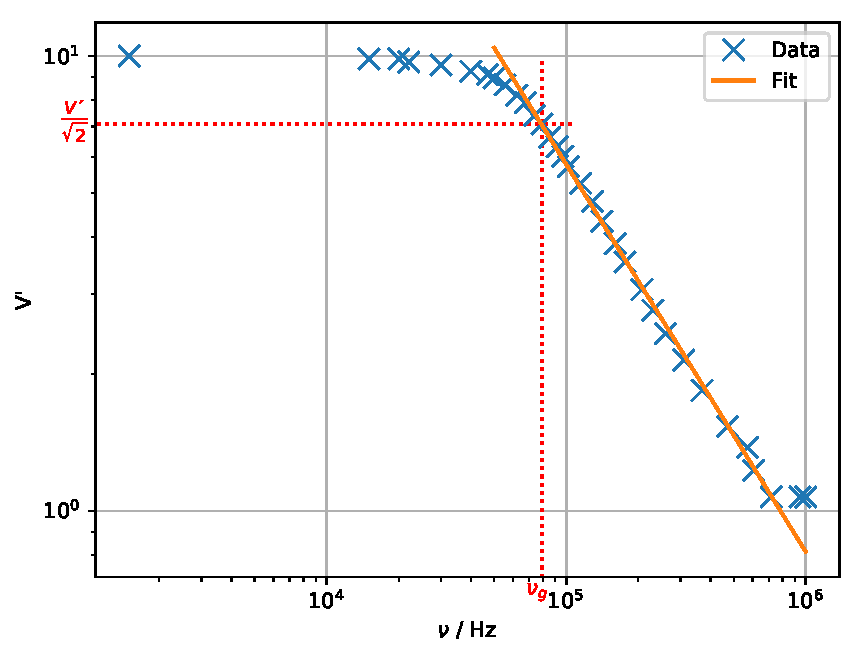
\includegraphics[scale=0.75]{plot1.pdf}
  \caption{Graphical representation of frequency response for $\frac{\text{R}_\text{N}}{\text{R}_\text{1}}$ = 10 ($V'_{10}$)} \label{fig:1}
\end{figure}
The fit curve is a fit of the function
\begin{equation*}
  f(x) = a\cdot x^b
\end{equation*}
and the parameters for $V'_{10}$ are
\begin{align*}
a &= (1.05\pm 0.11)\cdot 10^5 \\
b &= -0.852\pm 0.009 \ .
\end{align*}
In addition the value for $\frac{V'_{10}}{\sqrt{2}} = \frac{10}{\sqrt{2}}$ and its corresponding frequency $\nu'_{g10} = (7.9 \pm 1.4)\cdot 10^4 Hz$ are marked
to compare these to the values for $V'_{100}$.
\begin{figure}[H]
  \centering
  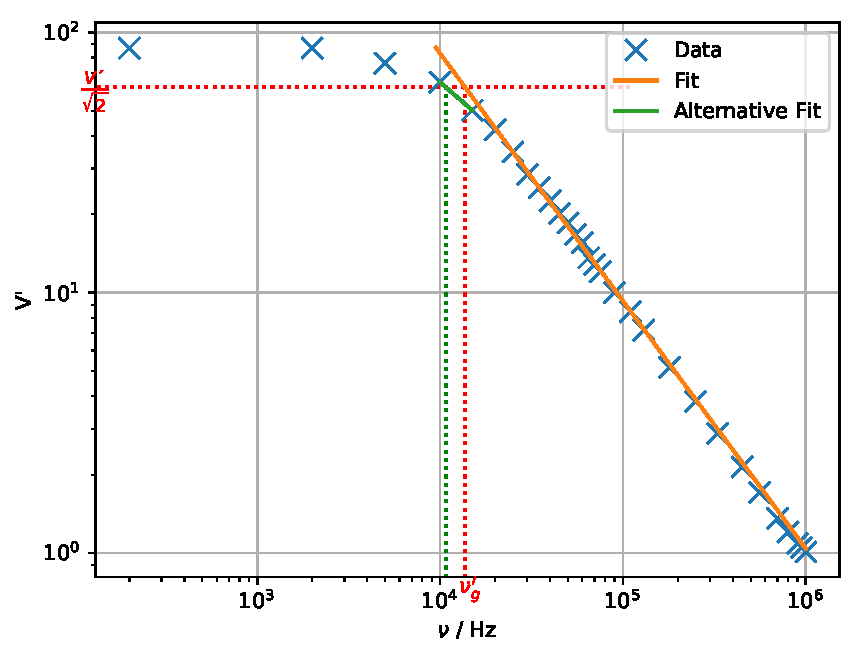
\includegraphics[scale=0.75]{plot3.pdf}
  \caption{Graphical representation of frequency response for $\frac{\text{R}_\text{N}}{\text{R}_\text{1}}$ = 100 ($V'_{100}$)} \label{fig:2}
\end{figure}
\noindent
The parameters for $V'_{100}$ are
\begin{align*}
a &= (5.3\pm 0.5)\cdot 10^5 \\
b &= -0.951\pm 0.009 \ .
\end{align*}
Here the marked value for $\frac{V'_{100}}{\sqrt{2}} = \frac{2}{0.023\cdot \sqrt{2}}$ with its frequency $\nu'_{g100} = (1.37 \pm 0.18)\cdot 10^4 Hz$ can now be
compared to the previous ones to verify the condition of the product of bandwidth and $V'$ being constant.
\begin{align*}
\nu'_{g10} V'_{10} &= (7.9\pm 1.4)\cdot 10^5 Hz \\
\nu'_{g100} V'_{100} &= (1.19+/-0.16)\cdot 10^6 Hz \\
\upDelta &= (51\pm 31) \%
\end{align*}
Looking at figure (\ref{fig:2}) it is clear, that the intersections of $\frac{V'_{100}}{\sqrt{2}}$ with the fitted curve and the direct connection between the data (visualized in green)
are about \SI{3}{\kilo\hertz} apart. This is why an alternative calculation $\nu'_{g100(alt)} V'_{100}$ with $\nu'_{g100(alt)} = \SI{10.8}{\kilo\hertz}$ (approximated through the graph) is done.
\begin{align*}
\nu'_{g10} V'{10} &= (7.9\pm 1.4)\cdot 10^5 Hz \\
\nu'_{g100(alt)} V'{100} &= 9.39\cdot 10^5 Hz \\
\upDelta_{alt} &= (19\pm 21) \%
\end{align*}

\subsection{Terminal Voltage}
The terminal voltage is measured with the inverting linear amplifier, $\nu = \SI{100}{\hertz}$ and a resistance ratio of $\frac{\SI{20}{\kilo\ohm}}{\SI{0.2}{\kilo\ohm}} = 100$ to
% \begin{equation*}
% U_T = \SI{360}{\milli\volt} \.
% \end{equation*}
If a resistance of $\SI{100}{\kilo\ohm}$ is switched in front of the amplifier, then the resistance ratio changes to $\frac{\SI{20}{\kilo\ohm}}{\SI{100.2}{\kilo\ohm}} = 100$ and it follows
\begin{equation*}
U_TR = \SI{15.7}{\milli\volt}
\end{equation*}
For the same procedure for the non-inverting electrometer (same resistance ratio and frequency) the results are
\begin{align*}
U_T &= \SI{3.8}{\volt} \\
U_{TR} &= \SI{3.8}{\volt} \ .
\end{align*}
Note that the absolute values are different due to the amplification done by the oscilloscope to get a visible signal without too much distortion, and only the
relation between the values is important.
The additional resistance has no effect on the electrometer but changes the outcome on the linear amplifier completely. This is because the linear amplifier has
a low input resistance (\approx $\text{R}_\text{1}$) and switching an additional one in series changes the total input resistance a lot. Therefore linear amplifier
is not suitable for measuring high-resistance voltage sources. However the electrometer has a relative high input resistance (\approx \SI{20}{\giga\ohm}) and does not
have these problems and can be used for measuring high-resistance voltage sources.

\subsection{Inverting Integrator}
In tabular (\ref{tab:int}) are the measured data for the inverting integrator.
\begin{table}[H]
  \centering
  \caption{Measurement Data for the inverting integrator} \label{tab:int}
  \pgfplotstabletypeset[
  col sep=semicolon,
  every head row/.style={
    before row={\toprule
    },
    after row=\hline
  },
  every last row/.style={after row=\bottomrule},
  columns/0/.style={column name=$\nu$ / Hz, column type=c },
  columns/1/.style={column name= $U_A$ / V, column type=c, precision=3},
  ]{integrator.csv}
\end{table}
\noindent
In figure (\ref{fig:int}) the data is visualized and the condition of $U_A \sim \frac{1}{\omega}$ can be verified. The operating range
ends approximately where the output voltage reaches a plateau value at about $\nu = \SI{1}{\kilo\ohm}$.
\begin{figure}[H]
\centering
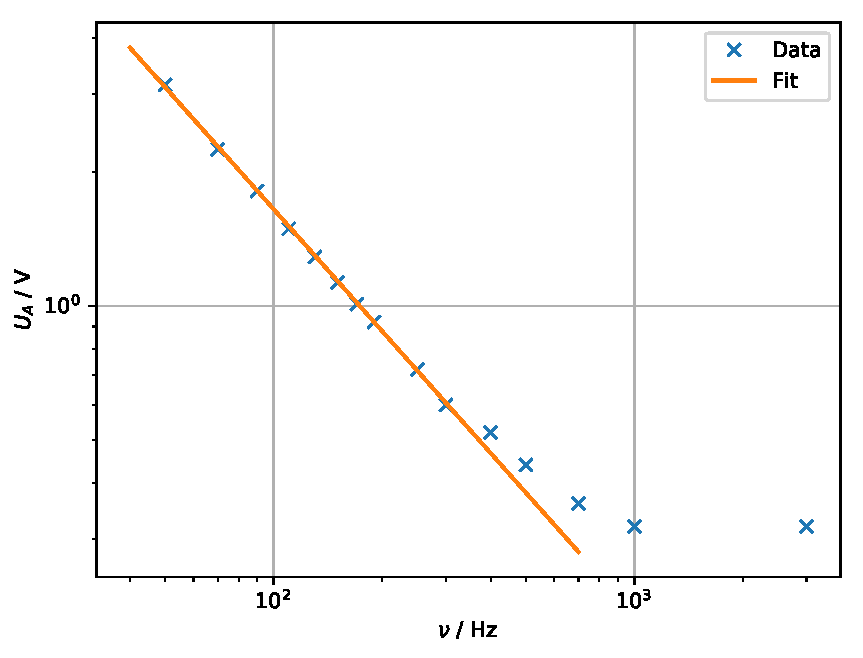
\includegraphics[scale=.75]{plot4.pdf}
\caption{Frequency response of the inverting integrator where $U_A \sim \frac{1}{\omega}$}\label{fig:int}
\end{figure}
\noindent
In figure (\ref{fig:int1}), (\ref{fig:int2}) and (\ref{fig:int3}) is a visualisation of how the inverting integrator works for
a sin voltage, triangular voltage and rectangular voltage.
\begin{figure}[H]
\centering
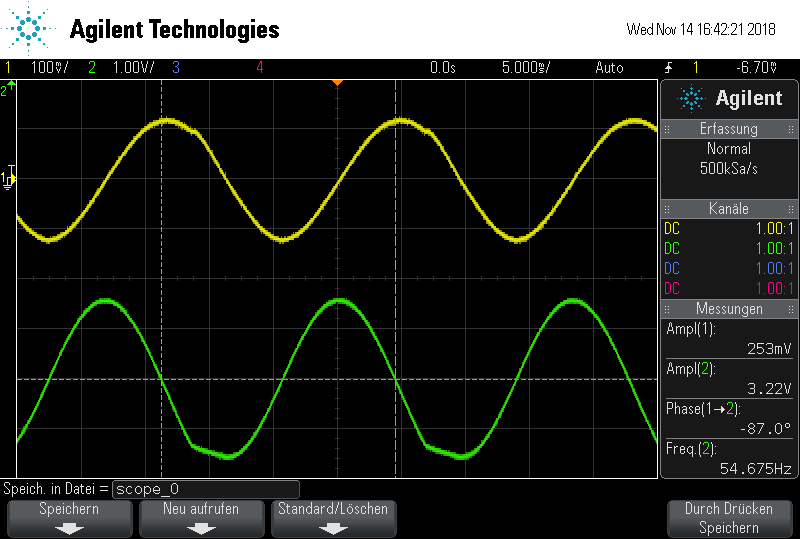
\includegraphics[scale=.48]{V51Bilder/inSin.png}
\caption{Sin voltage integrated}\label{fig:int1}
\end{figure}
\begin{figure}[H]
\centering
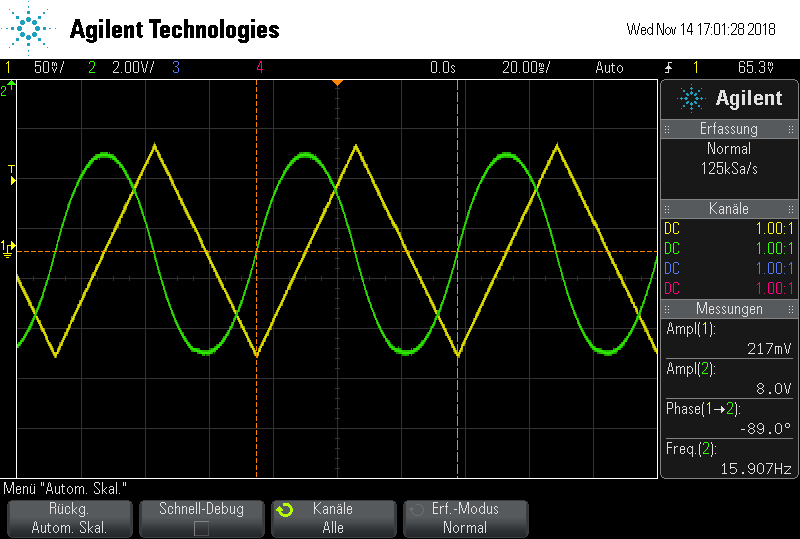
\includegraphics[scale=.48]{V51Bilder/intTri.png}
\caption{Triangular voltage integrated}\label{fig:int2}
\end{figure}
\begin{figure}[H]
\centering
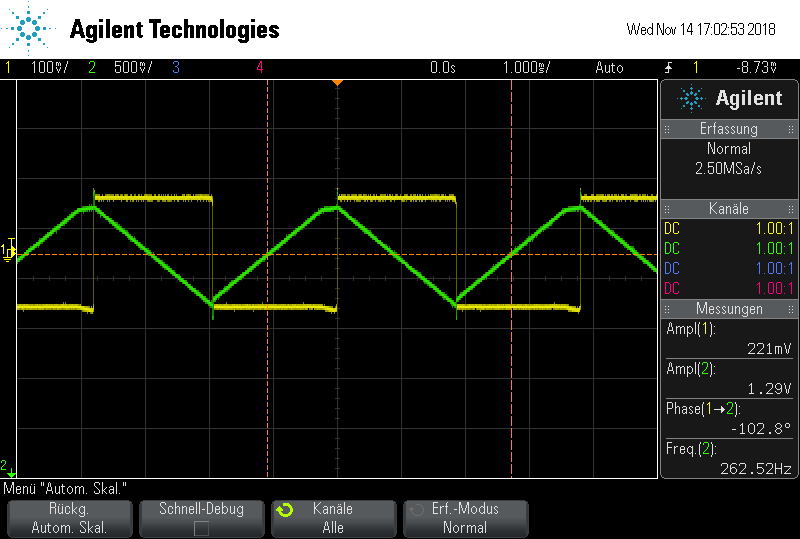
\includegraphics[scale=.48]{V51Bilder/intRect.png}
\caption{Rectangular voltage integrated}\label{fig:int3}
\end{figure}


\subsection{Inverting Differentiator}
In tabular (\ref{tab:diff}) are the measured data for the inverting differentiator.
\begin{table}[H]
  \centering
  \caption{Measurement Data for the inverting differentiator} \label{tab:diff}
  \pgfplotstabletypeset[
  col sep=semicolon,
  every head row/.style={
    before row={\toprule
    },
    after row=\hline
  },
  every last row/.style={after row=\bottomrule},
  columns/0/.style={column name=$\nu$ / Hz, column type=c, },
  columns/1/.style={column name= $U_A$ / mV, column type=c, precision=3},
  ]{differentiator.csv}
\end{table}

\begin{figure}[H]
\centering
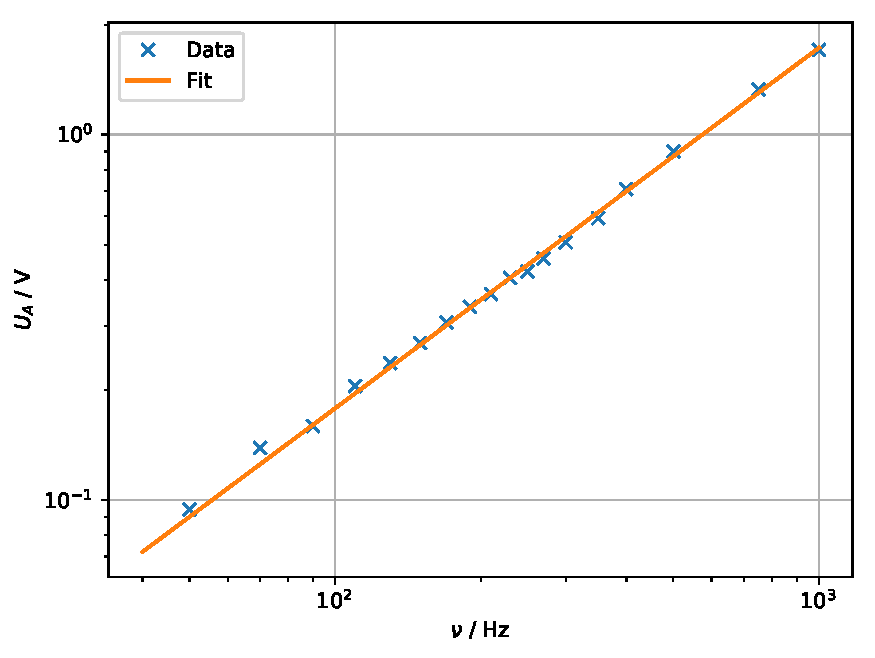
\includegraphics[scale=.75]{plot5.pdf}
\caption{Frequency response of the inverting differentiator where $U_A \sim \omega$}\label{fig:dif}
\end{figure}
\noindent
As no meaningful discrepancy of the fitted curve and the data points is seen, the condition $U_A \sim \omega$ applies for the
whole operating range that has been examined. \\ \noindent
In figure (\ref{fig:diff1}), (\ref{fig:diff2}) and (\ref{fig:diff3}) is a visualisation of how the inverting differentiator works for
a sin voltage, triangular voltage and rectangular voltage.
\begin{figure}[H]
\centering
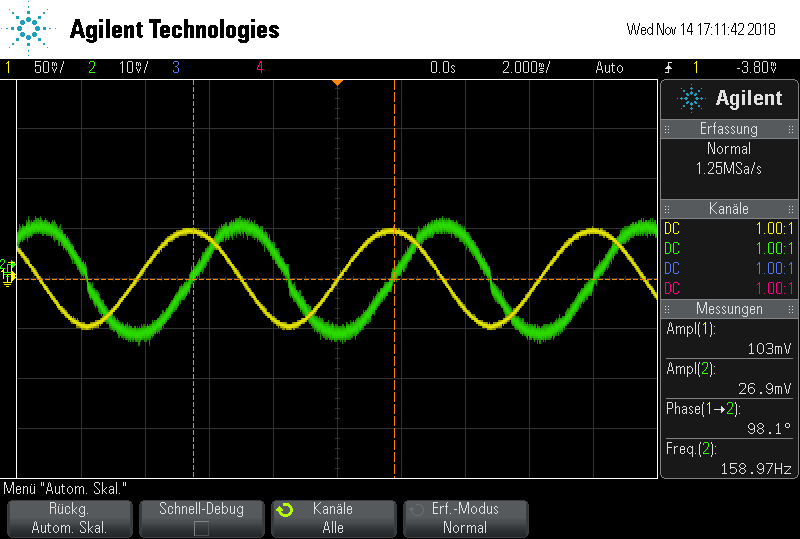
\includegraphics[scale=.48]{V51Bilder/diffSin.png}
\caption{Sin voltage differentiated}\label{fig:diff1}
\end{figure}
\begin{figure}[H]
\centering
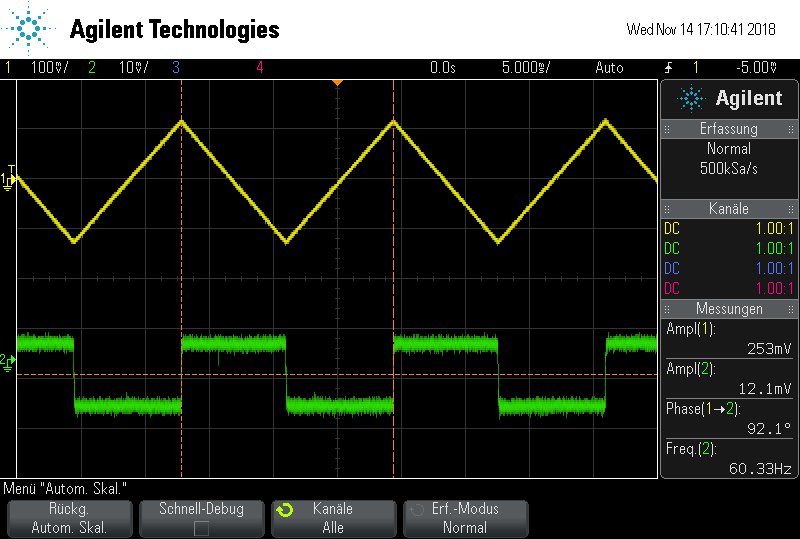
\includegraphics[scale=.48]{V51Bilder/diffTri.png}
\caption{Triangular voltage differentiated}\label{fig:diff2}
\end{figure}
\begin{figure}[H]
\centering
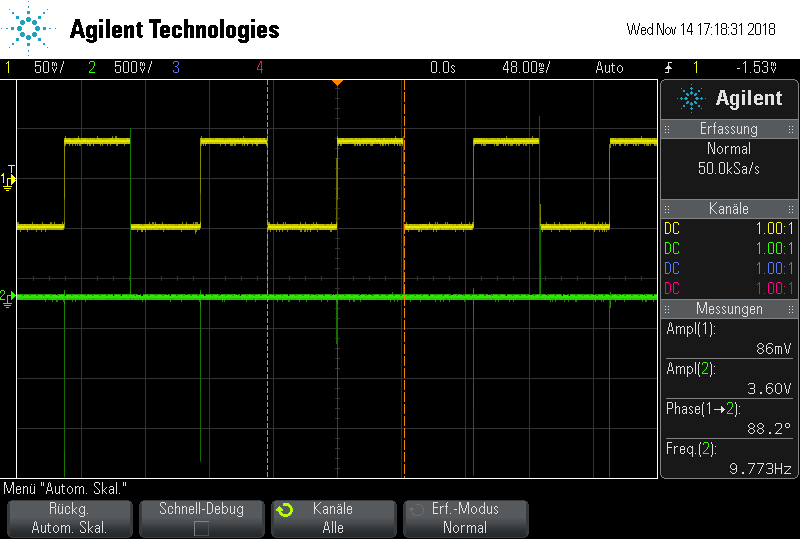
\includegraphics[scale=.48]{V51Bilder/diffRect.png}
\caption{Rectangular voltage differentiated (notice the green spikes)}\label{fig:diff3}
\end{figure}

\subsection{Schmitt-Trigger}
For a resistance ratio of $\frac{\text{R}_\text{1}}{\text{R}_\text{P}} = \frac{\SI{10}{\kilo\ohm}}{\SI{100}{\kilo\ohm}}$ the measurement
for the trigger voltage $U_{B(trigger)}$ and the voltage $2U_B$ gives
\begin{align*}
U_{B(trigger)} &= \SI{1.405}{\volt} \\
2U_B &= \SI{26.9}{\volt} \ .
\end{align*}
The difference between $\frac{\text{R}_\text{1}}{\text{R}_\text{P}}U_B = \SI{1.345}{\volt}$ and $U_{B(trigger)}$ is \SI{4.5}{\percent}.
To see the Schmitt-Trigger in action the trigger effect is visualised in figure (\ref{fig:trig})
\begin{figure}[H]
  \centering
  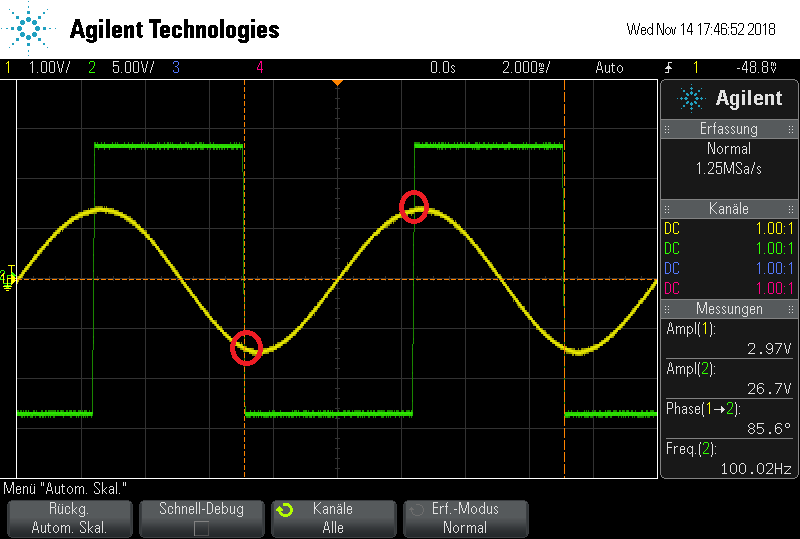
\includegraphics[scale=.9]{V51Bilder/schmitt.png}
  \caption{Visualisation of the trigger effect at a Schmitt-Trigger. (yellow=input, green=output)} \label{fig:trig}
\end{figure}
\noindent
The red circles mark the spots where the input voltage reaches $\pm \frac{\text{R}_\text{1}}{\text{R}_\text{P}}U_B$. Notice
that, once triggered, the output voltage keeps the same as long as the input voltage does not reach the opposing trigger voltage.
Inbetween lies the switch hysterese.

%\section{Discussion}
The frequency responses measured with the linear amplifier cover the expected form of the theory. For $V'_{10}$ at low frequencies the neutral amplification
has to be very large, because the amplification of the measurement and the expected value from the resistance ratio are exactly the same. This means that the used precision
of the measurement in millivolts was not enough to get a difference between the resistance ratio and $V'$, as it is supposed in equation (\ref{eq:3}). In contrast to that for $V'_{100}$
a neutral amplification of $V = 666.67$ was approximated. This value is quite low for the neutral amplification of an operation amplifier that usually are very large values of about $10^5$ or even higher.
Therefore this is probably not a precise approximation. \\
\newline
\noindent
The product of bandwidth and $V'$ is supposed to be constant, but had differences between the two measurements, respectively between the two fitted curves, of  $\Delta = (51 \pm 31)\%$. That is
a relatively big range, caused by the errors of the fit, with a possible minimum of $\Delta_{min} = \SI{20}{\percent}$. Looking at the figure of $V'_{100}$ it was already mentioned, that the fitted curve does not cover the
data in the inspected range that precisely. \\
To clarify that the real frequency $\nu'_g$ is probably shifted to the left the alternative calculation, where $\frac{V'}{\sqrt{2}}$ exactly cuts the direct connection between the
data, lead to $\Delta = (19 \pm 21)\%$. This is still a relatively big range but obviously closer to the condition of a constant product. \\
Further the product $\nu'_{g100} V'_{100} = (1.19+/-0.16)\cdot 10^6 Hz$ is the transit frequency, but looking at the graph it is clear that the fitted curve cuts the point where $V'_{100} = 1$ much more left.
This is one more reason to expect the actual $\nu'_g$ to be shifted to the left. \\
For the transit frequency $\nu'_{g10} V'_{10} = (7.9\pm 1.4)\cdot 10^5 Hz$ for $V'_{10}$ in contrast the calculated value and the graph cover each other nicely.
Concluding this it is verified, that the operational amplifier works more stable at low amplifications.\\
\newline
\noindent
The different measurements of the terminal voltage verify as expected, that the linear amplifier is not suited for measuring high-resistance voltage sources, as the output signal is easily influenced by changes
of the input resistance. However the electrometer amplifier showed no difference, whether there was an additional input resistance or not, and therefore is suited much better for these kinds of measurement. \\
\newline
\noindent
The conditions, $U_A \sim \frac{1}{\omega}$ for the inverting integrator and $U_A \sim \omega$ for the inverting differentiator, were both verified. For the inverting integrator the operating range could be limited
to about $<\SI{3}{\kilo\hertz}$ but for the inverting differentiator no such limit was found, probably because not enough frequency range was covered in the measurement. \\
The thermal prints of both show very nicely how the circuit is able to integrate/differentiate (and invert) different input signals.\\
\newline
\noindent
For the last part with the Schmitt-Trigger, the trigger function, adjusted by the resistance ratio, and its relation to the operating voltage $\pm U_B$ were verified
and the thermal print very nicely underlines and visualises the effect.

\printbibliography{}
\end{document}
